\documentclass[a4paper,11pt]{beamer}
\usepackage[utf8]{inputenc}
\usepackage{lmodern}
\usepackage{caption}
\usepackage{subcaption}
% Thème Darmstadt
\usetheme{Darmstadt}
\usepackage{graphicx}
\usepackage{ragged2e}
\usepackage{listings}
\usepackage{color}
\usepackage{libs/gitdags}
\usepackage{fontawesome, wasysym}
\usepackage{tikz}
\usepackage{grafcet}
\usepackage{algorithm}
\usepackage{algpseudocode}
%\captionsetup[figure]{labelformat=empty}

\setbeamertemplate{navigation symbols}{} 
\setbeamertemplate{footline} 
{  
	\begin{beamercolorbox}[ht=2.5ex,dp=1.125ex,%
      leftskip=.3cm,rightskip=.3cm plus1fil]{title in head/foot}%
      {\usebeamerfont{title in head/foot}\insertshorttitle} \hfill    
      \insertframenumber / \inserttotalframenumber%
    \end{beamercolorbox}%
%     \begin{beamercolorbox}[colsep=1.5pt]{lower separation line foot}
%     \end{beamercolorbox} 
}

% Informations sur la présentation
\title{Travaux pratiques Informatique Embarquée}
\author{} 
\institute{Université de Toulon\\IUT GEII Première année}
\date{}

\newcounter{exampleBlockCounter}
\setcounter{exampleBlockCounter}{1} 

\definecolor{comment}{rgb}{0.12, 0.38, 0.18 } %adjusted, in Eclipse: {0.25, 0.42, 0.30 } = #3F6A4D
\definecolor{keyword}{rgb}{0.37, 0.08, 0.25}  % #5F1441
\definecolor{string}{rgb}{0.06, 0.10, 0.98} % 

\lstset{
language=C,
frame=single,
frameround=tttt,
rulesepcolor=\color{black},
showspaces=false,showtabs=false,tabsize=2,
numberstyle=\tiny,numbers=left,
stringstyle=\color{string},
keywordstyle = \color{keyword}\bfseries,
commentstyle=\color{comment}\itshape,
basicstyle=\ttfamily\footnotesize,
breaklines=true,
captionpos=b
}

%\includeonlyframes{current}

\begin{document}

% Première diapositive : Titre
\begin{frame}[plain]
    \titlepage
    \center{\includegraphics[scale=0.75]{images/by-nc-sa.eps}}
	\vspace{1.2cm}
	\center{
\includegraphics[scale=0.111]{images/logo-utln.eps} \hspace{1cm}
	\includegraphics[scale=0.0825]{images/logogeii.eps}}
    
\end{frame}

\begin{frame}{TPs Informatique Embarquée}
	\tableofcontents[hideallsubsections]
\end{frame}

\AtBeginSection{%
    \begin{frame}
        \tableofcontents[sections=\value{section}]
    \end{frame}
}

\section{Introduction}
\subsection{Présentation}
\begin{frame}
\center{frank.buloup@univ-amu.fr}
\end{frame}
\subsection{Organisation}
\begin{frame}
\begin{block}{Séances de TPs}
	\begin{itemize}
		\item Mardi aprèm
		\item 9 de 3h (13h30-16h30) et 2 de 1h30 (13h30-15h)
		\item Travail en monômes
		\item Vous pouvez vous aider et demander de l'aide !
	\end{itemize}
\end{block}

\begin{alertblock}{Il y a des règles durant ces séances !}
	\begin{itemize}
		\item Si pas de carte alors pas de TP !
		\item Pas de téléphone : éteint dans le sac
		\item Pas d'IA durant les séances
		\item Lors de l'évaluation, vous n'aurez pas accès aux outils d'IA
	\end{itemize}
\end{alertblock}

\end{frame}


\section{La carte XIAO SAMD21 et sa programmation}
\subsection{Vue d'ensemble de la carte}
\begin{frame}

\center{\includegraphics[scale=0.25]{images/xiao-pinout.eps}}

\textcolor{blue}{\textbf{\underline{\href{https://docs.arduino.cc/language-reference/}{Arduino language Ref.}}}}	



\end{frame}
\subsection{Le Main}
\begin{frame}

\center{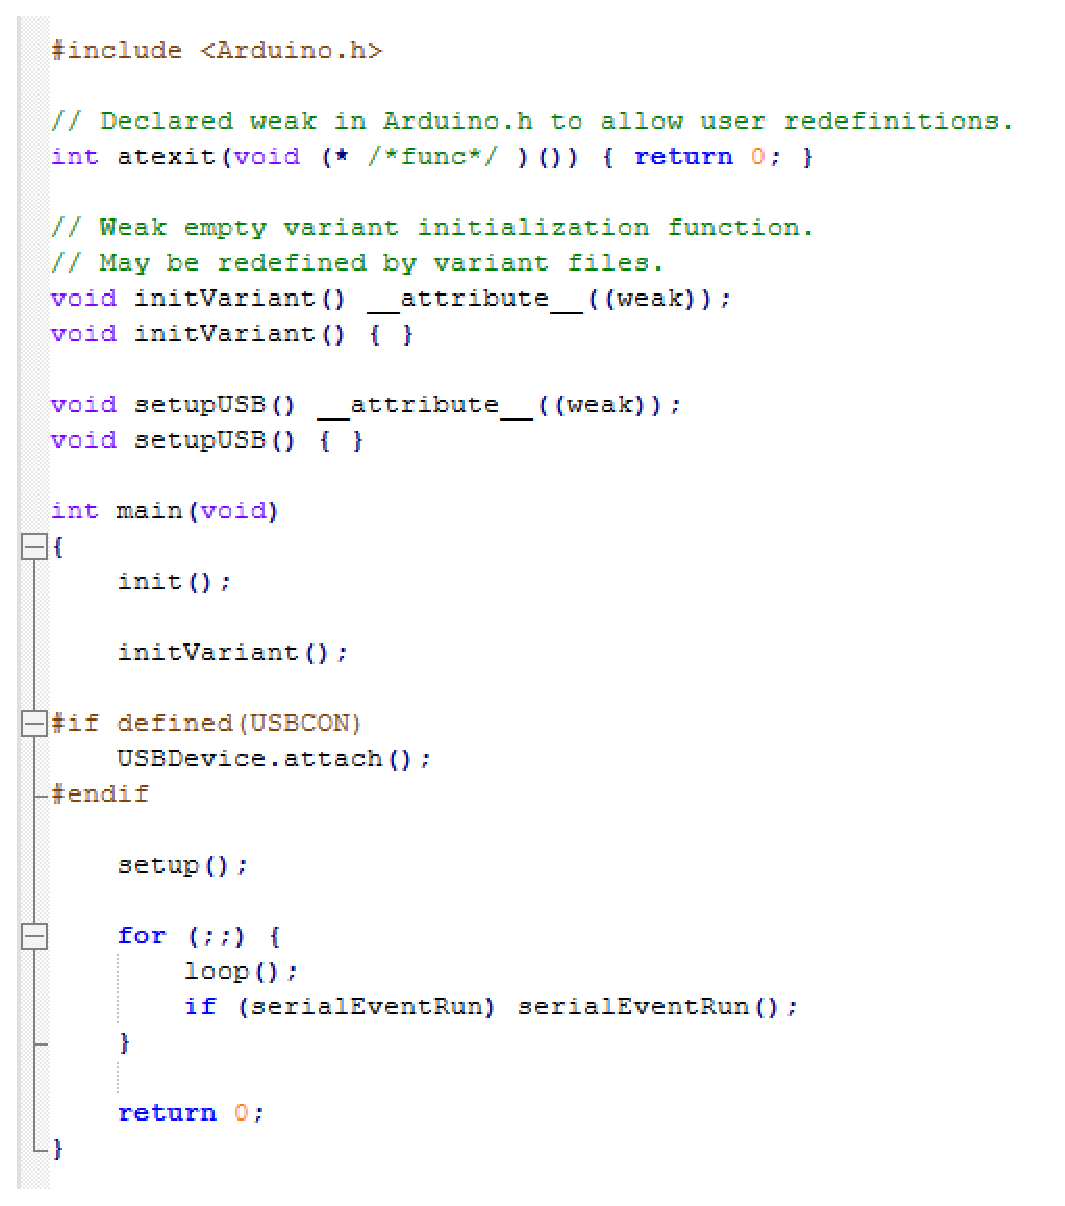
\includegraphics[scale=0.4]{images/Main.eps}}

\end{frame}

\begin{frame}

\begin{alertblock}{La fonction \textbf{loop()}}
	\begin{itemize}
		\item Le nom \textbf{loop()} est mal choisi !
		\item C'est un "faux ami"
		\item C'est une fonction pas une boucle !
		\item Mais cette fonction est bien appelée dans une boucle \textbf{for(;;)}
		\item Et cette boucle n'a pas de fin d'exécution : boucle infinie !
	\end{itemize}
\end{alertblock}

\end{frame}

\subsection{Les entrées/sorties numériques}
\begin{frame}
\center{\includegraphics[scale=0.2]{images/digitalwrite.eps}}
\end{frame}

\begin{frame}
\center{\includegraphics[scale=0.2]{images/digitalRead.eps}}
\end{frame}

\subsection{Les entrées/sorties analogiques}
\begin{frame}
\center{\includegraphics[scale=0.2]{images/analogWrite.eps}}
\end{frame}
\begin{frame}
\center{\includegraphics[scale=0.2]{images/analogRead.eps}}
\end{frame}

\subsection{Système temps réel}
\begin{frame}


\end{frame}

\section{Exemples d'implémentation d'un GRAFCET}
\subsection{Exemple général}

\begin{frame}
\begin{figure}
   \includegraphics[width=0.4\textwidth]{images/grafcet.eps}
   \includegraphics[width=0.575\textwidth]{images/CCode.eps}
\end{figure}
\end{frame}

\subsection{Application TP1}
\begin{frame}
\begin{figure}
   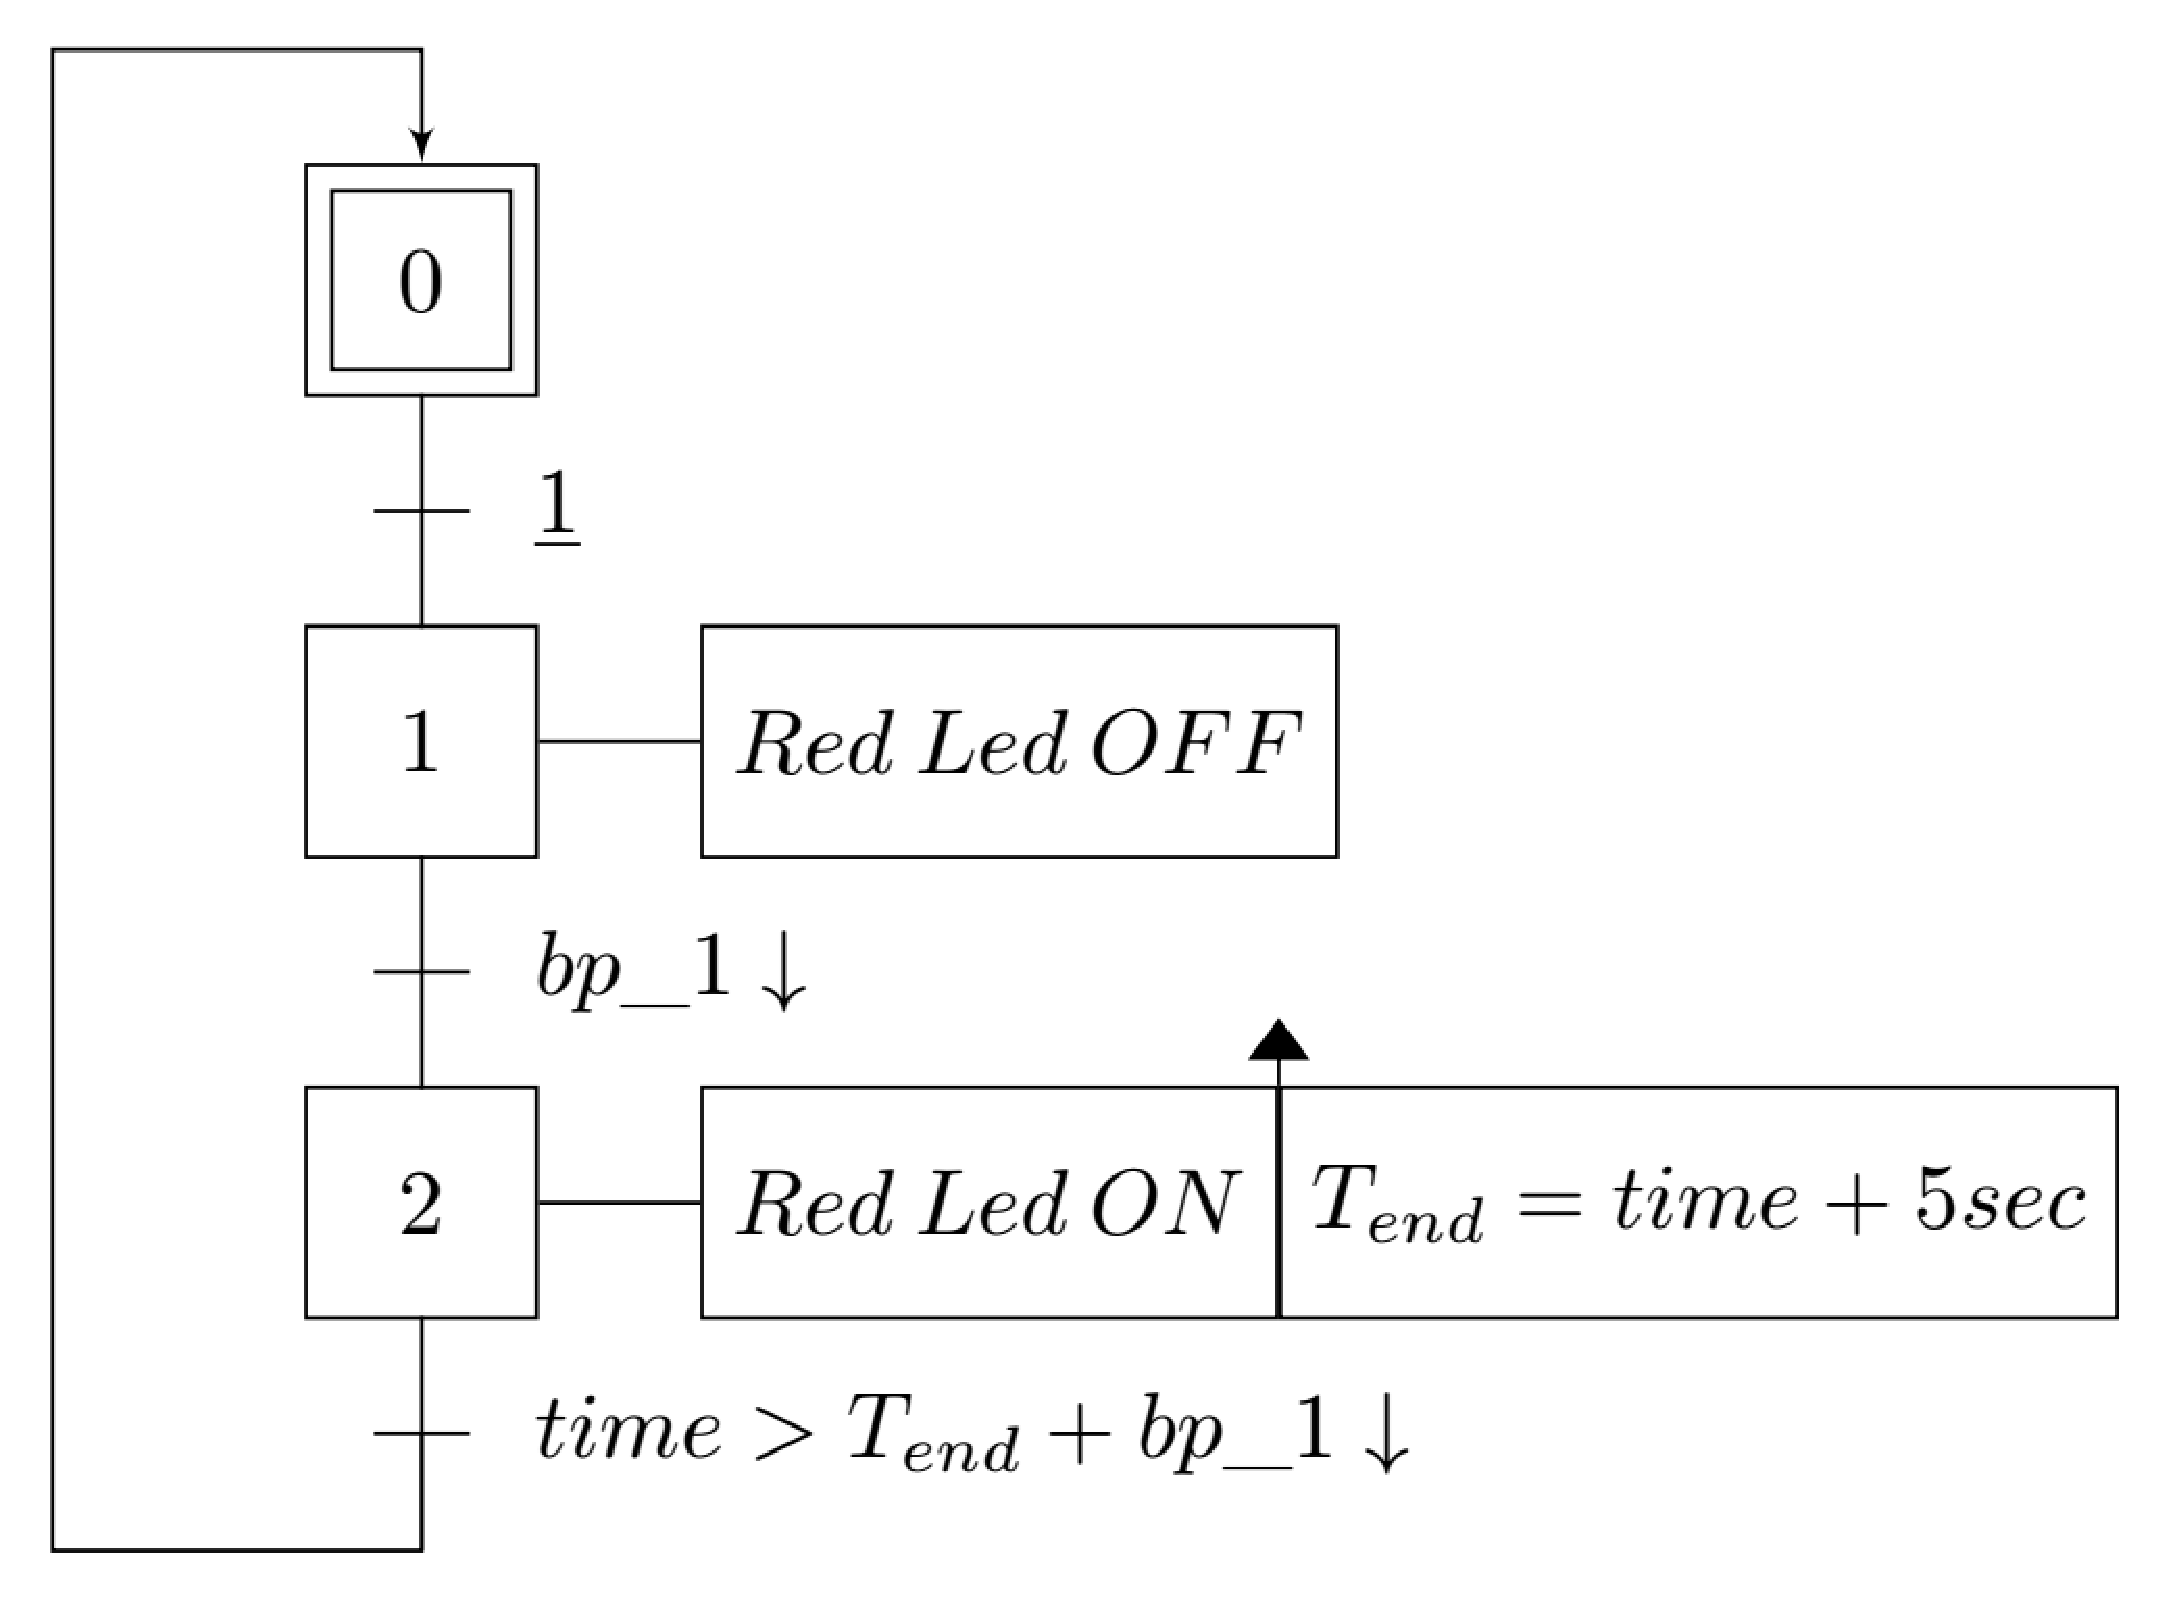
\includegraphics[width=0.4\textwidth]{images/Grafcet_Prog8_1.eps}
   \vspace{.5cm}
   
   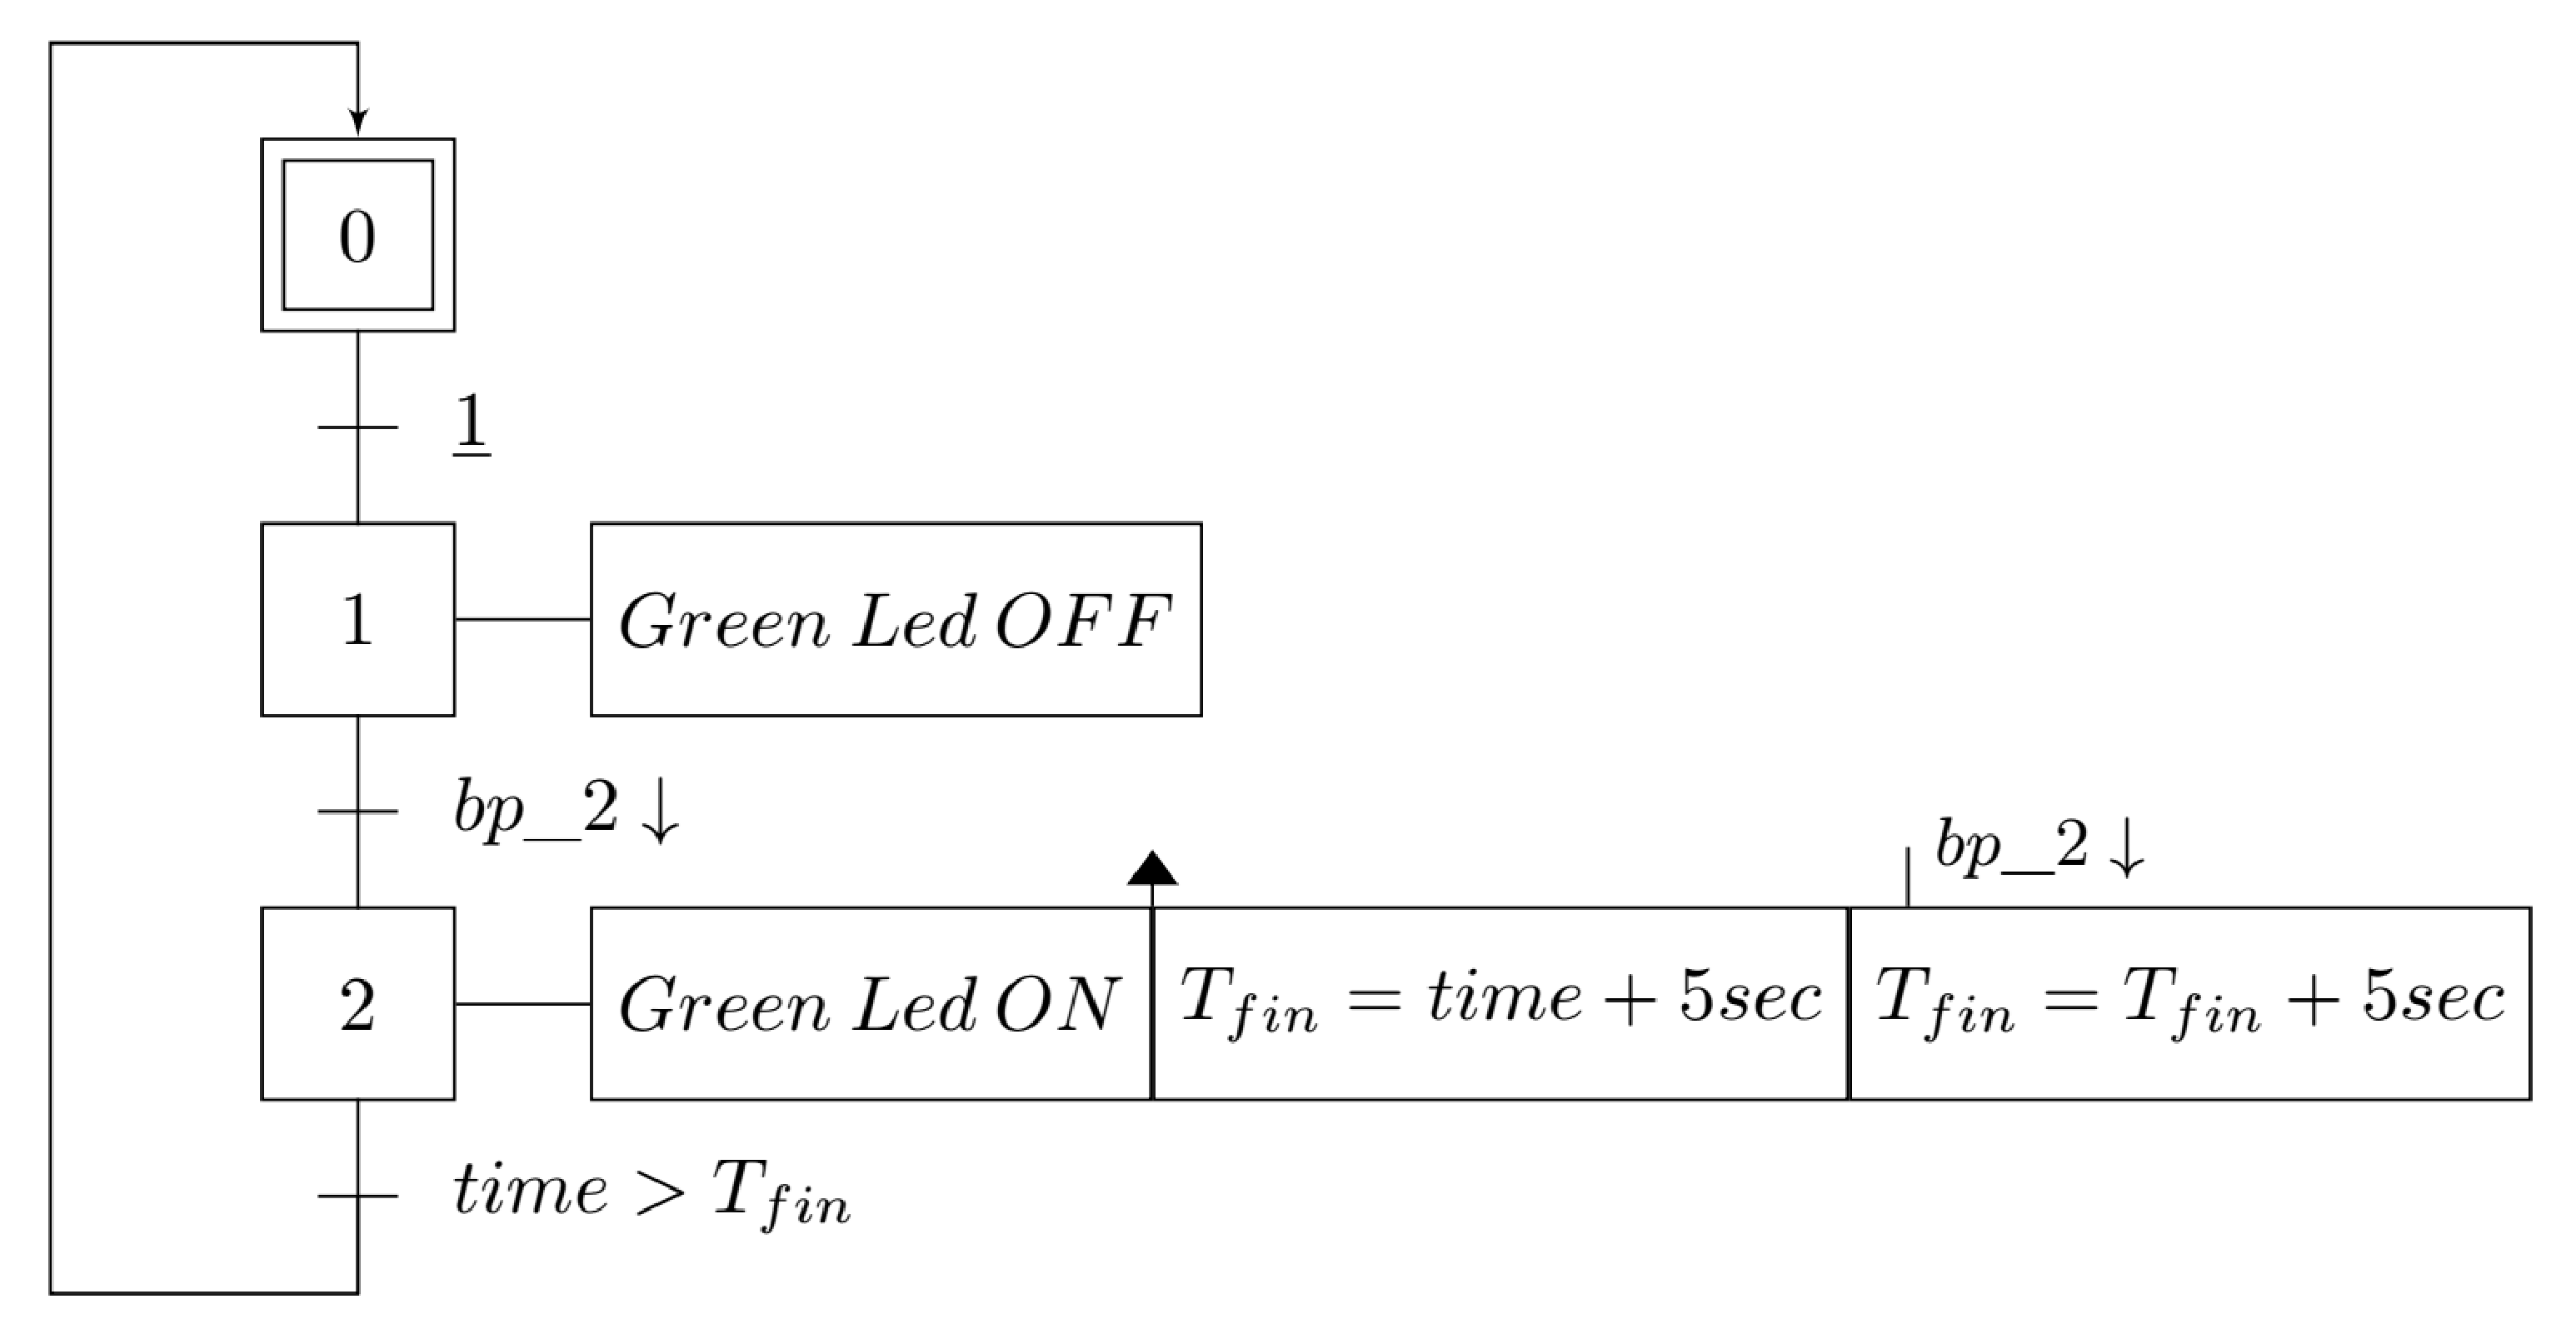
\includegraphics[width=0.575\textwidth]{images/Grafcet_Prog8_2.eps}
\end{figure}
\end{frame}




\end{document}





